
\begin{figure}[H]
    \centering
    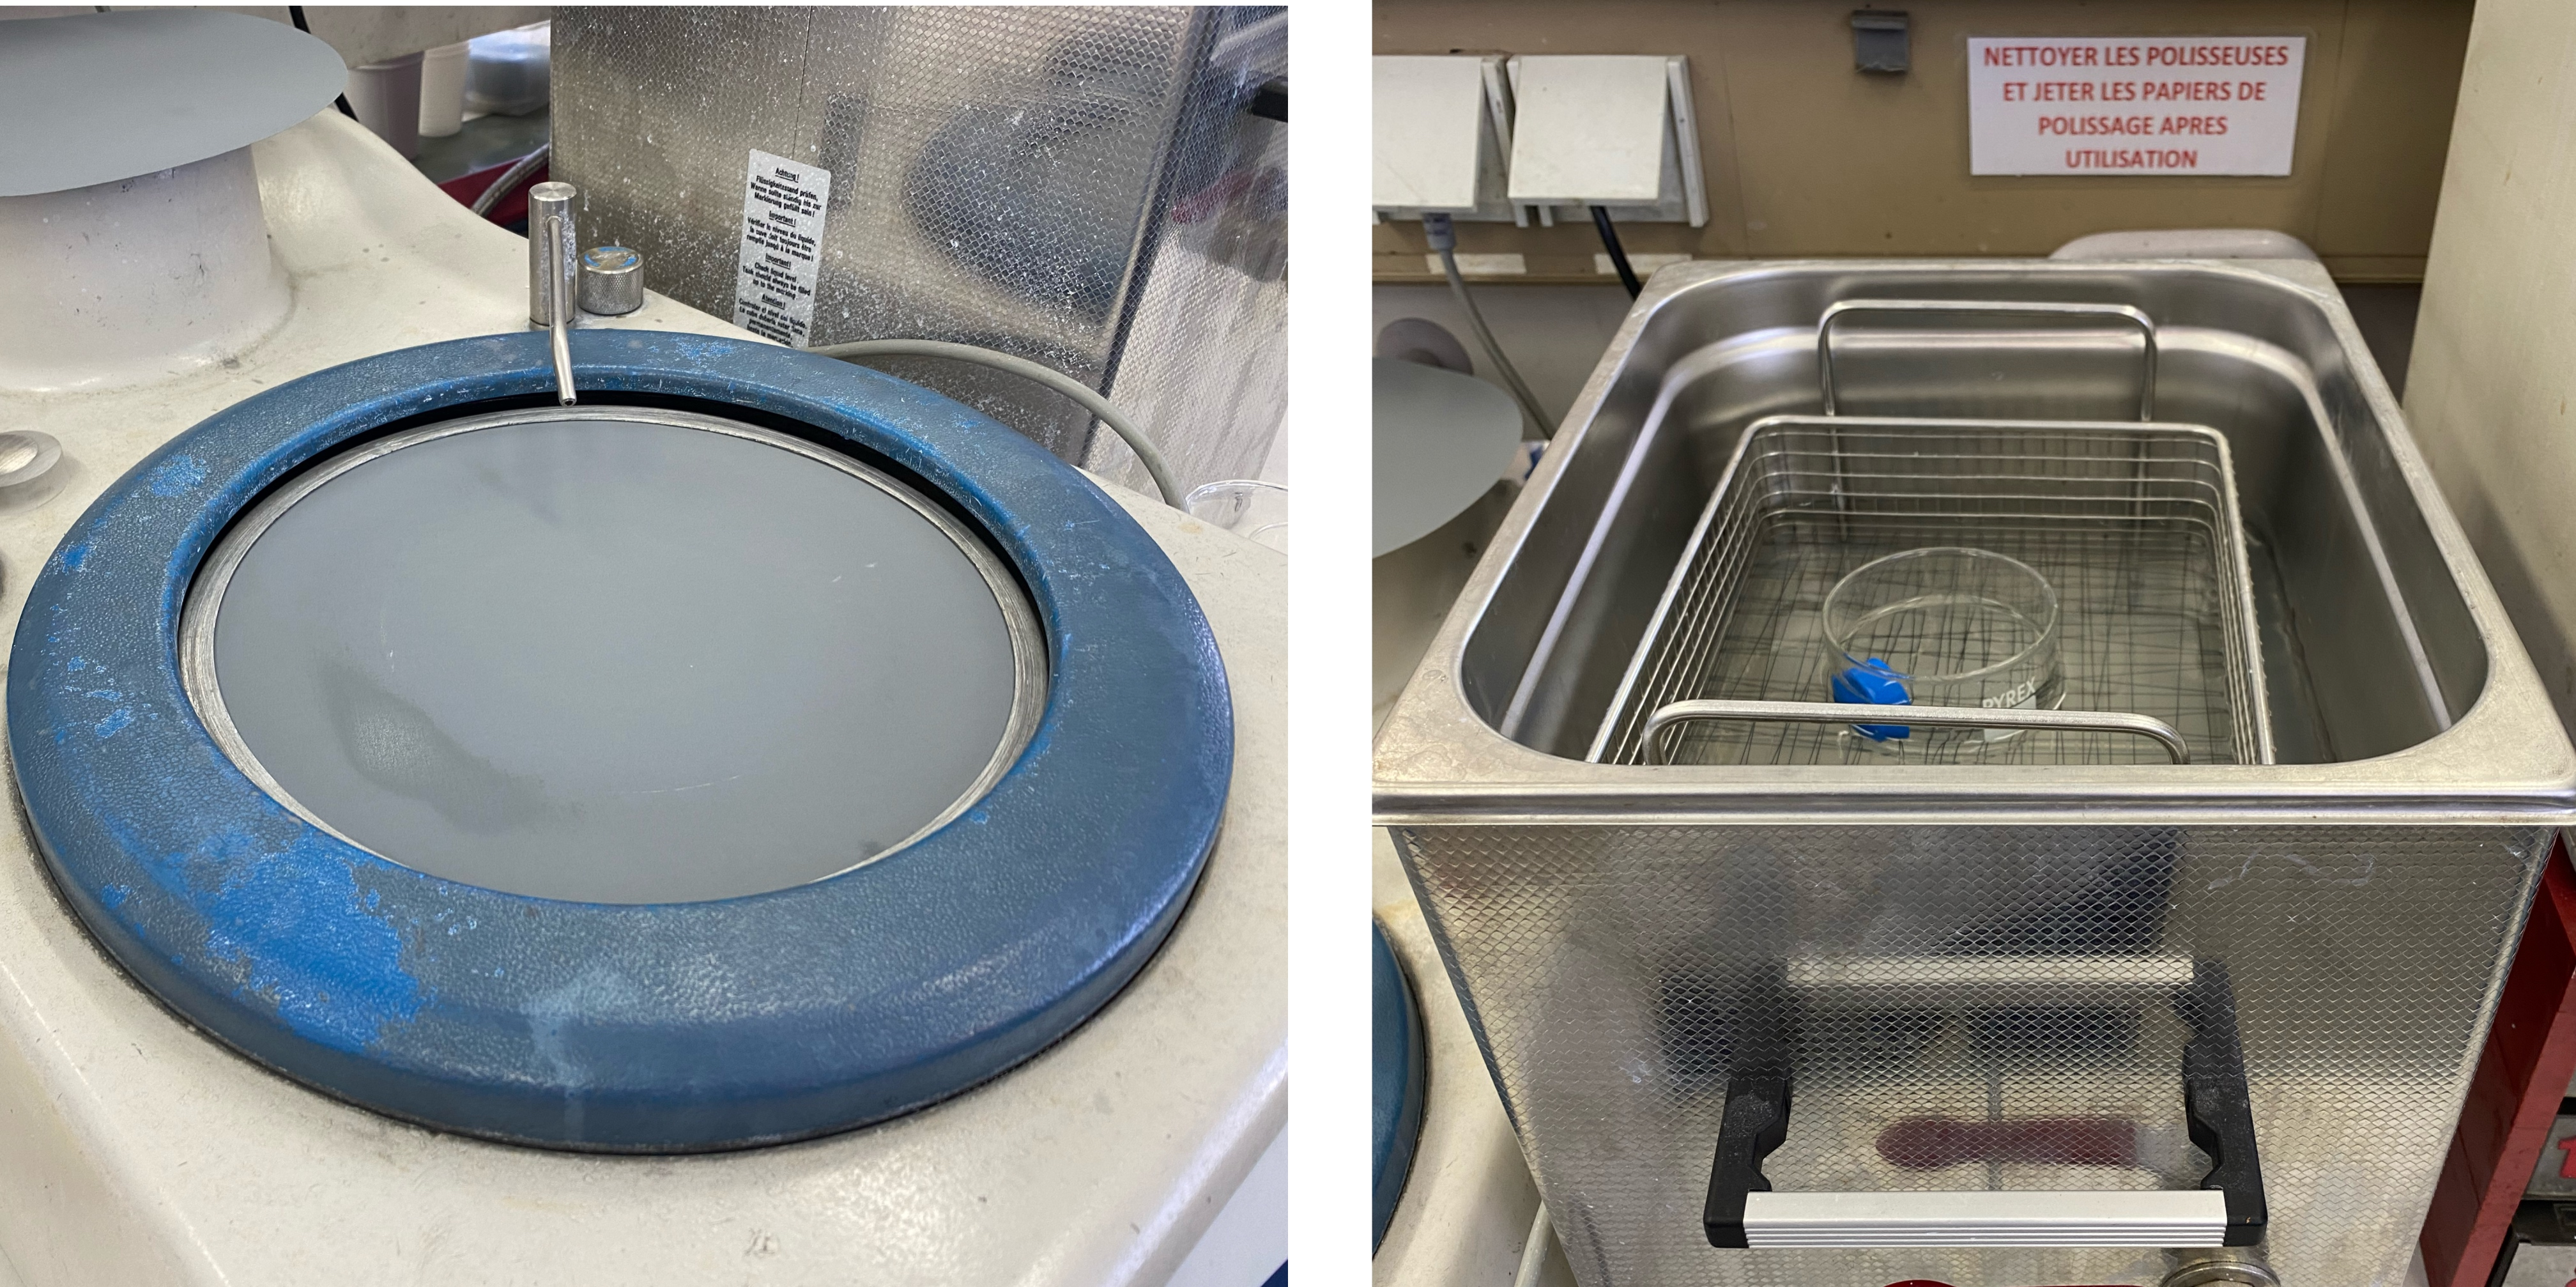
\includegraphics[width=0.55\textwidth]{images/WechatIMG1126.jpeg}
    \caption{Polisseur tournant et bain à ultrasons}
    \label{fig:polisseur_bain_ultrasons}
\end{figure}


L'étape de polissage et nettoyage est cruciale pour ne pas avoir 
trop de défauts à la surface de l'échantillon:
on polit la pièce sur un polisseur tournant (grain de 1200 puis de 2400, lubrifié par l'eau),
puis on la passe au bain à ultrasons 2 minutes pour la nettoyer.
Ensuite polit à 2µm et 1µm avec une autre machine et un lubrifiant spécifique,
puis on repasse au bain à ultrasons pour finir de la nettoyer.\\


\begin{figure}[H]
    \centering
    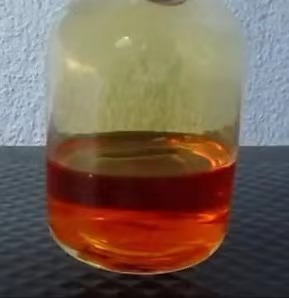
\includegraphics[width=0.3\textwidth]{images/WechatIMG1128.jpeg}
    \caption{La solution d'eau régale prête à l'emploi}
    \label{fig:eau_regale}
\end{figure}


On utilise un mélange composé de deux tiers d'acide chlorhydrique 
et d'un tiers d'acide nitrique.
On attend 2 minutes que les deux acides réagissent ensemble.
On observe que la solution passe de transparente à jaune-orangée.
On peut ensuire faire tremper les pièces 45 secondes chacune dans la solution, 
le but étant qu'elles soient suffisamment attaquées pour révéler les dendrites, 
mais de ne pas dissoudre une épaisseur trop importante.\\


\begin{figure}[H]
    \centering
    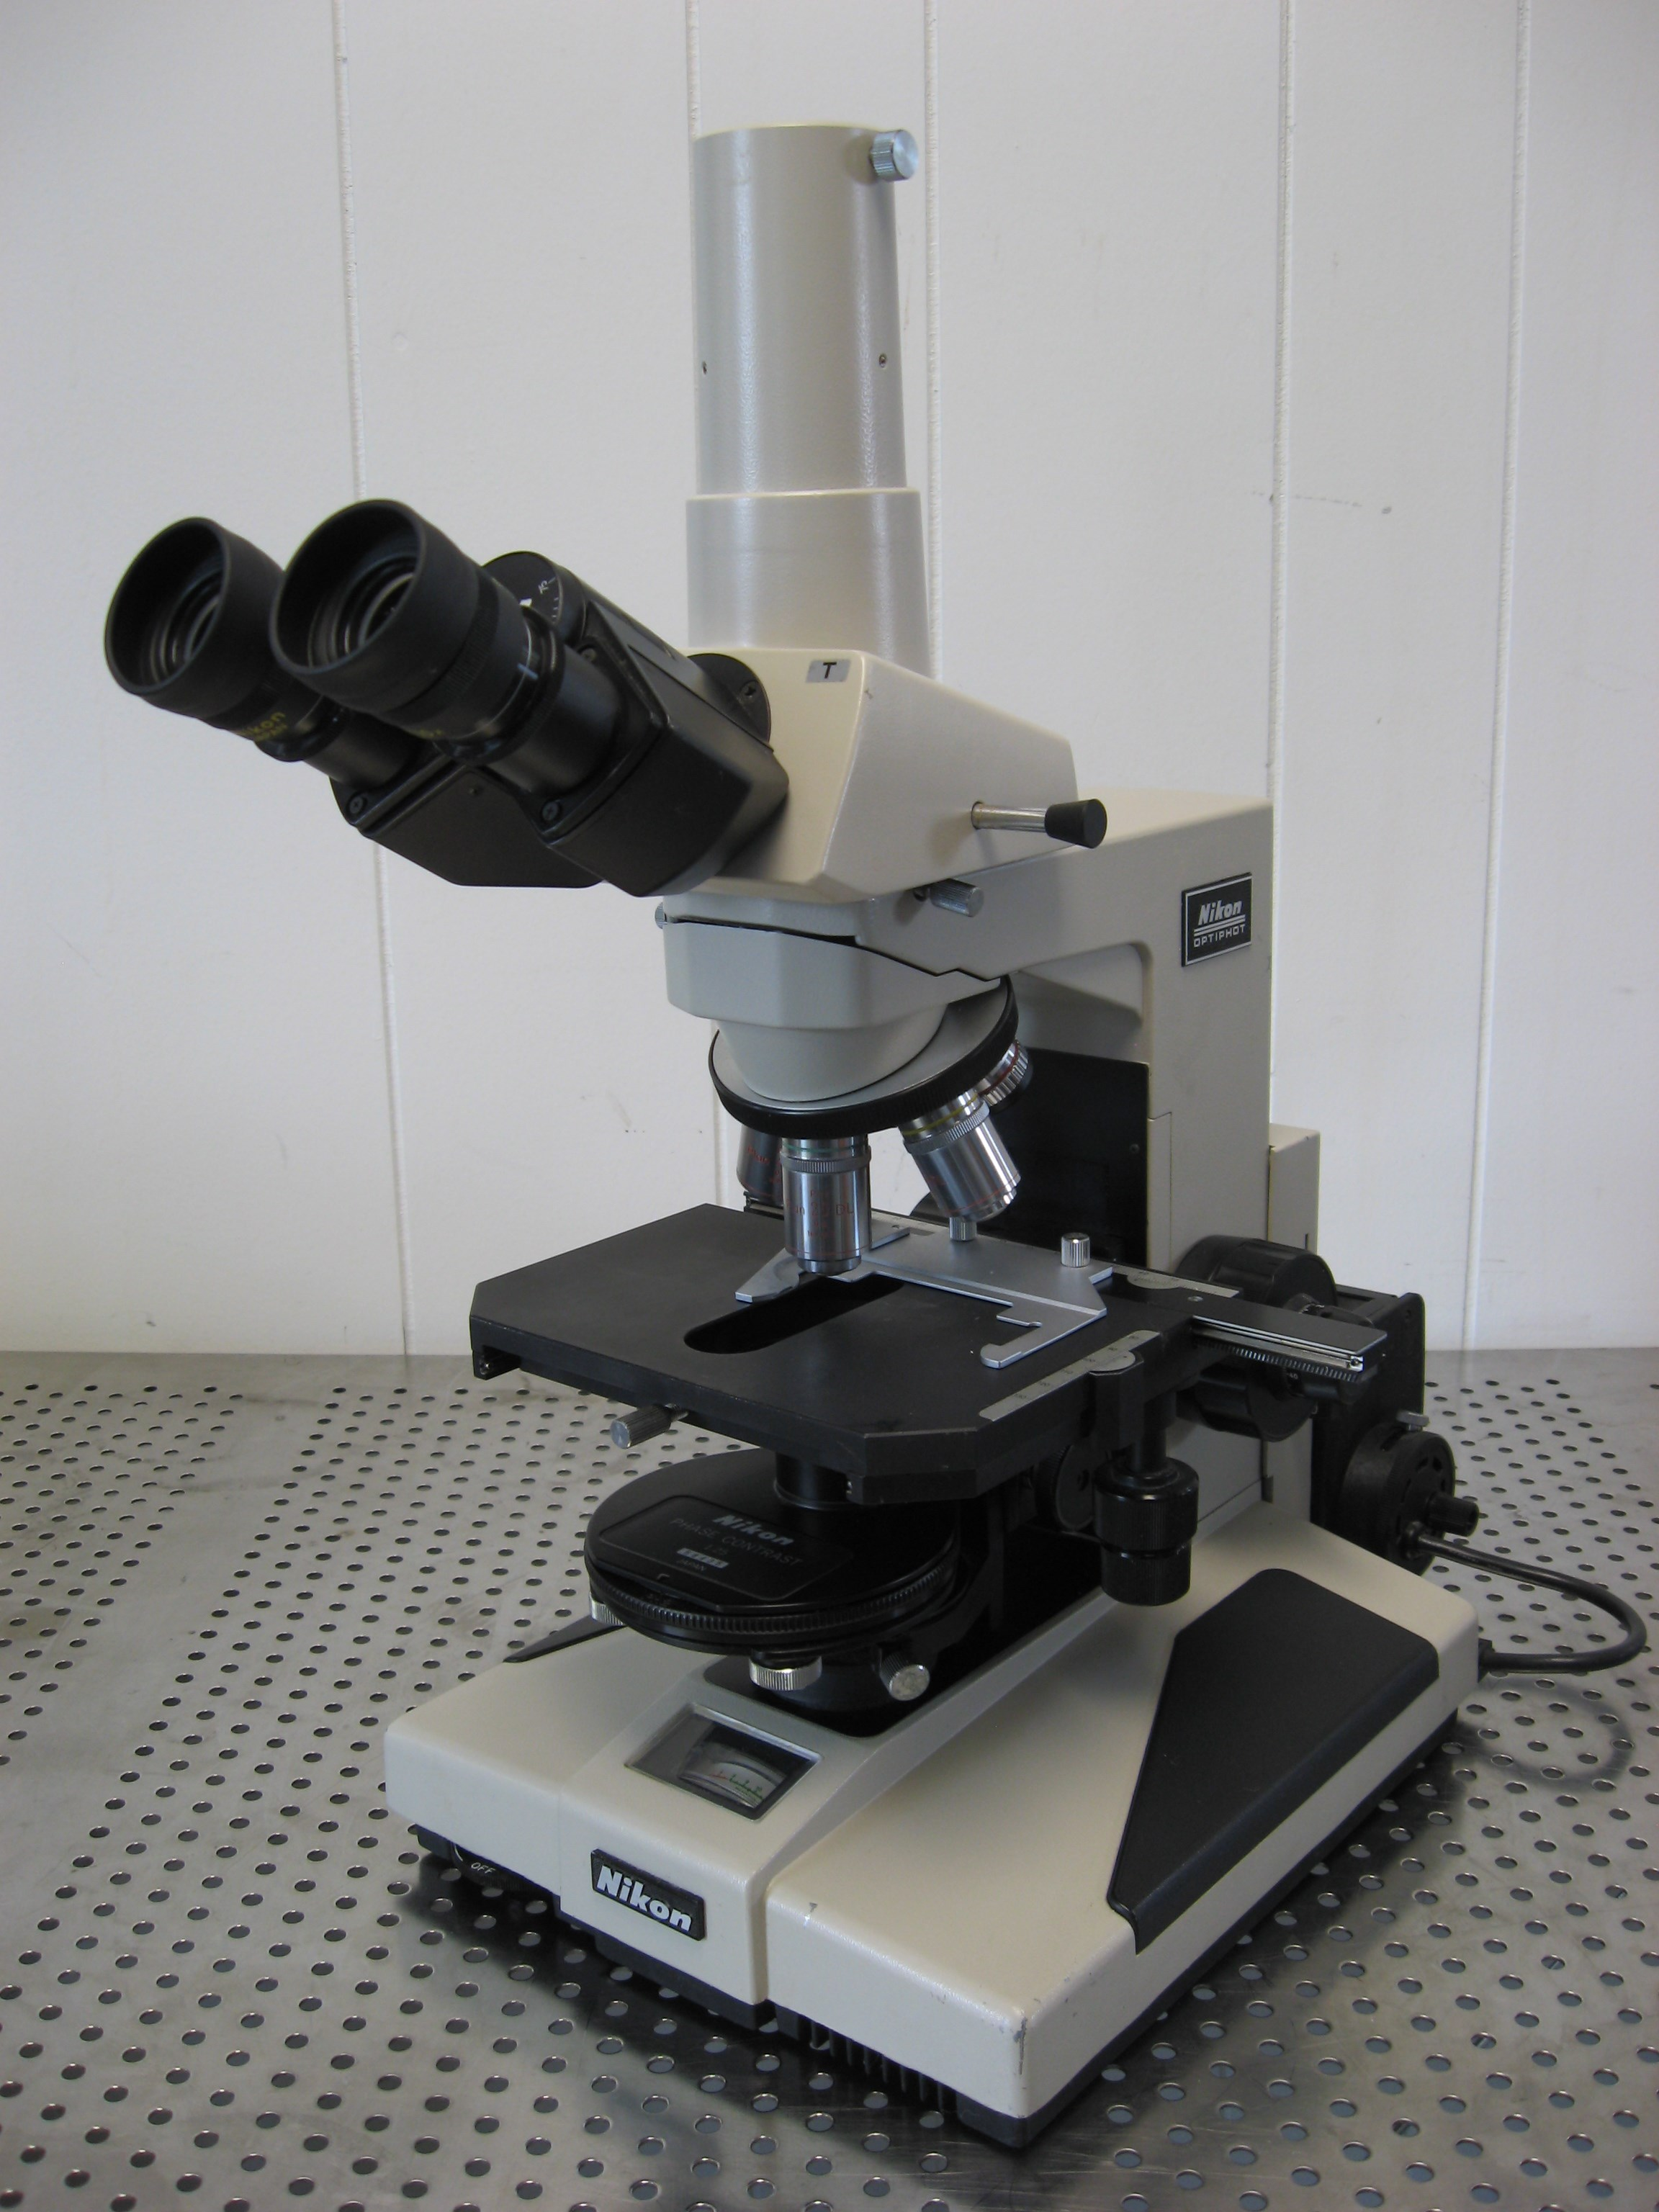
\includegraphics[width=0.35\textwidth]{images/optique.jpg}
    \caption{Le microscope optique utilisé pour examiner la surface des échantillons}
    \label{fig:microscope_optique}
\end{figure}


Le microscope optique permet d'observer nos échantillons à l'échelle de la centaine 
de \SI{}{\micro\metre} ce qui permet de rapidement repérer les défauts les plus gros 
tels que les pores ou les fissures.\\


\begin{figure}[H]
    \centering
    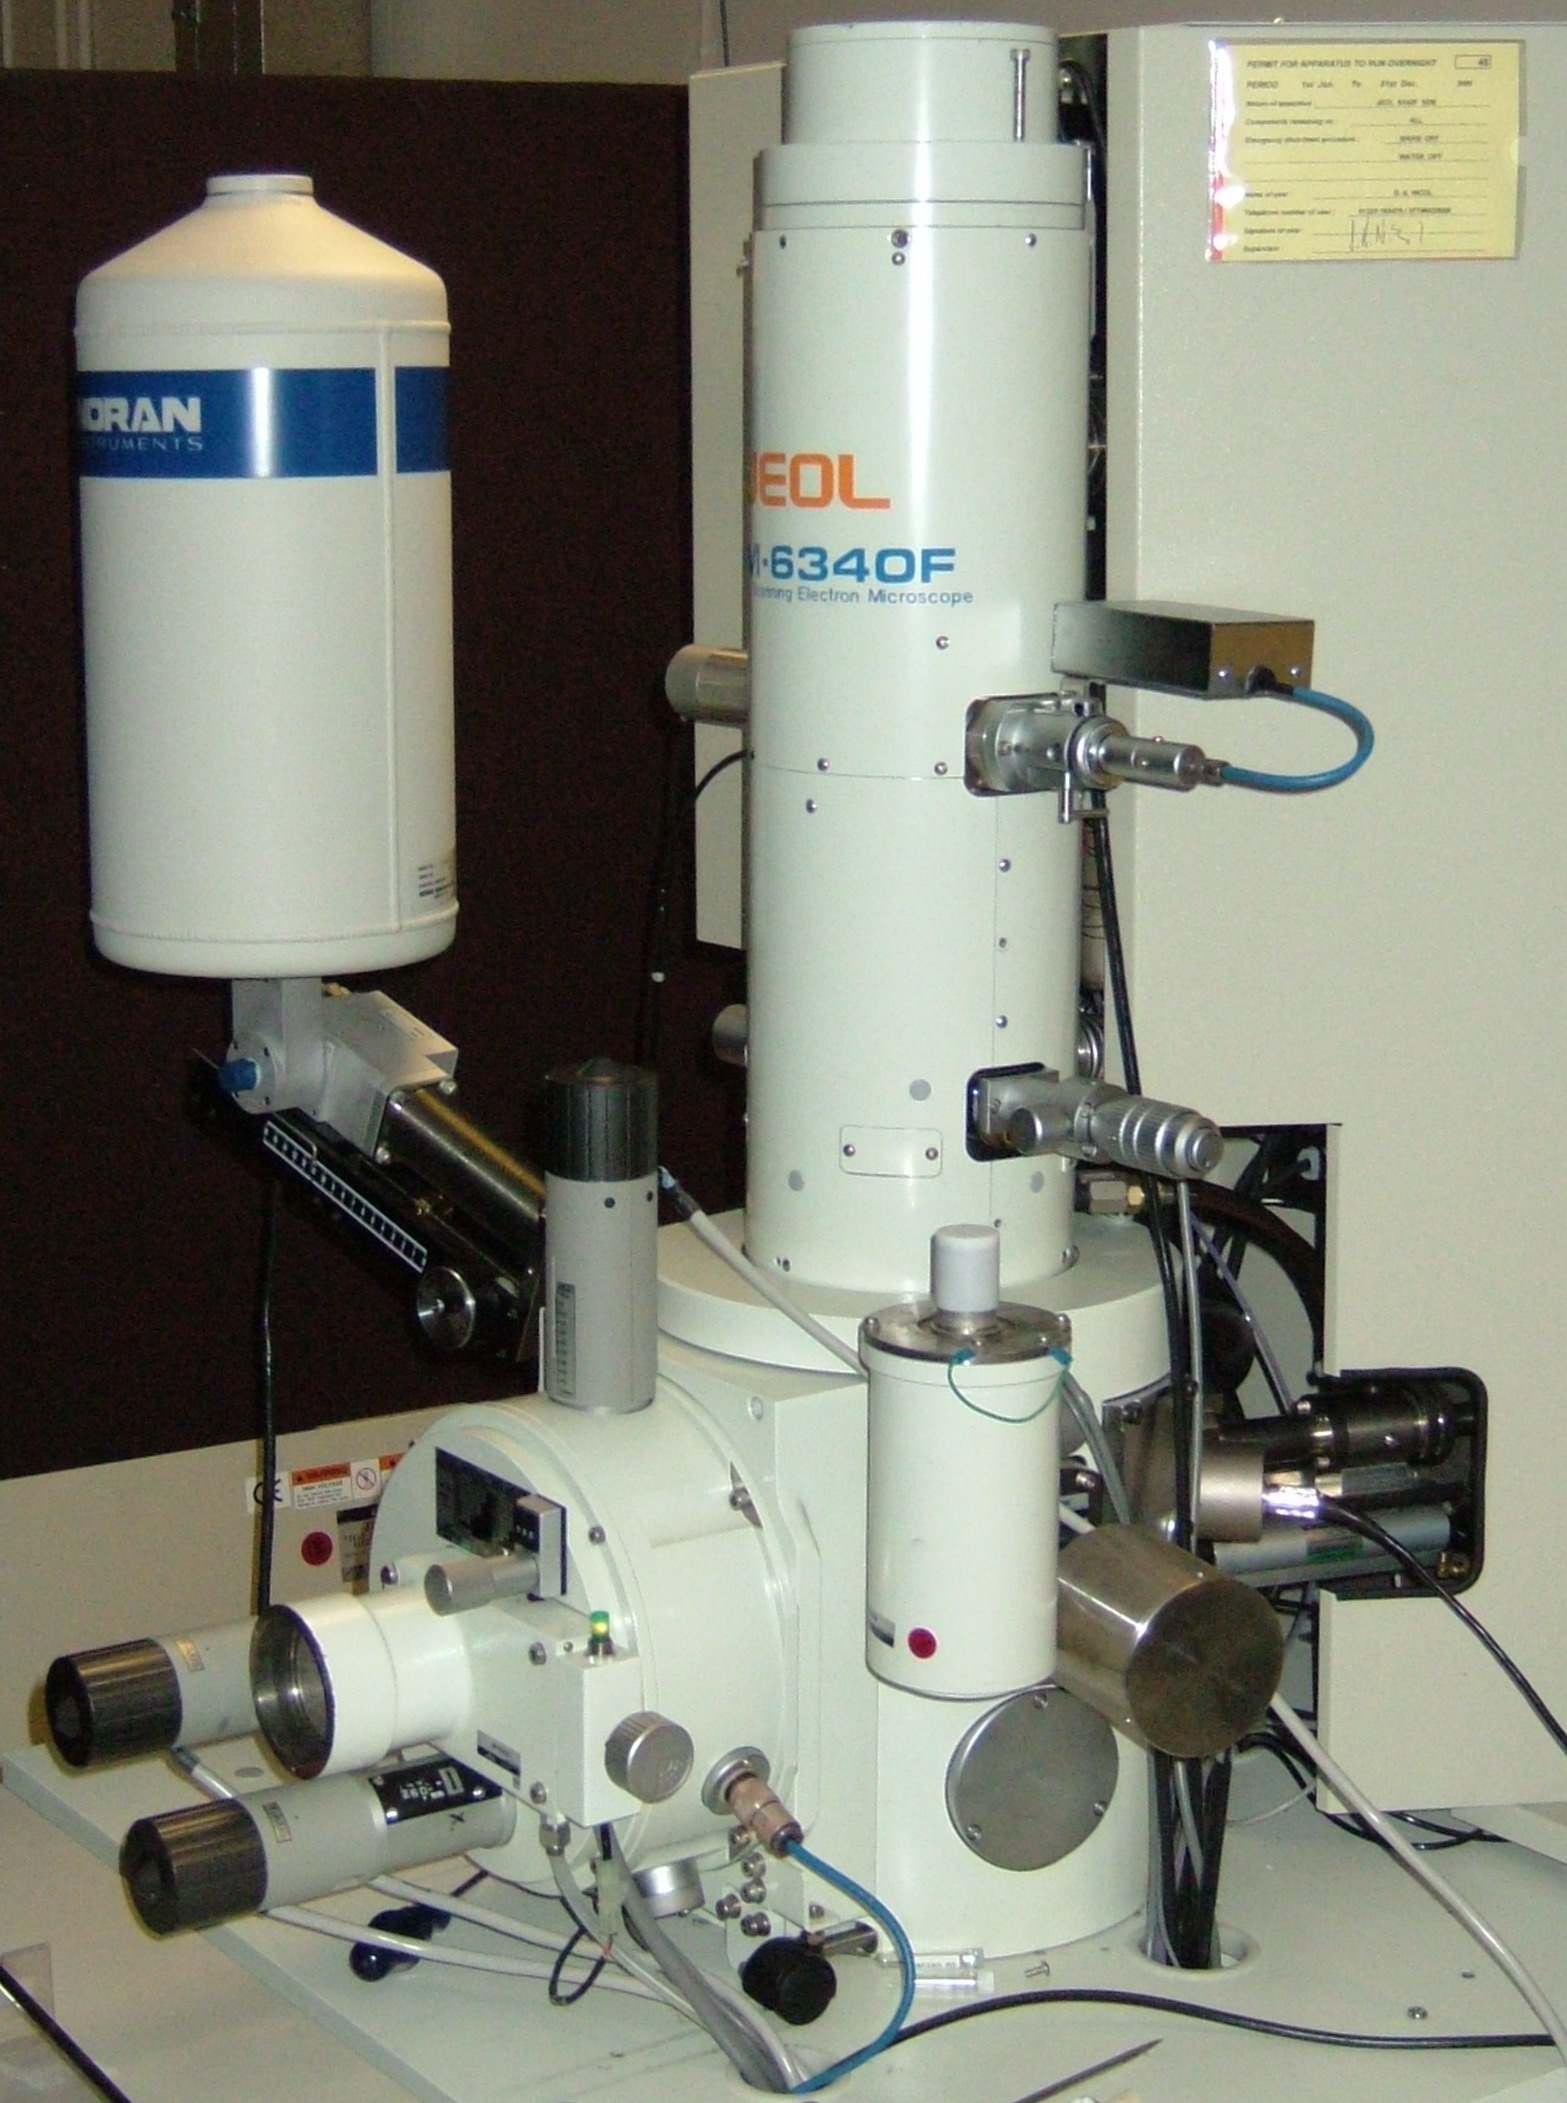
\includegraphics[width=0.4\textwidth]{images/JEOL_JSM-6340F.jpg}
    \caption{Microscope électronique à balayage pour observer la microstructure des échantillons}
    \label{fig:MEB}
\end{figure}


Des observations au MEB (microscope électronique à balayage) sont réalisées.
Le microscope optique ne nous permettait pas d'observer l'influence 
du traitement thermique sur l'agencement des phases $\gamma$ et de $\gamma'$. La résolution
du MEB de l'ordre du \SI{}{\micro\metre} nous permet d'observer la phase $\gamma'$ dans la matrice
$\gamma$ ainsi que les éventuels agrégats eutectiques. La détection d'électrons rétro-diffusés
permet de plus de voir à l'image les phases $\gamma$ et $\gamma'$. En effet, les atomes légers
de la phase $\gamma'$ sont moins déviés que les atomes plus lourds de la phase $\gamma$. Ainsi
les couloirs de matrice $\gamma$ apparaissent en blanc et la phase $\gamma'$ apparaît en noir.

